\chapter{Execution on the Robot}
\label{chap:Execution on the robot}
\begin{figure}[H]
    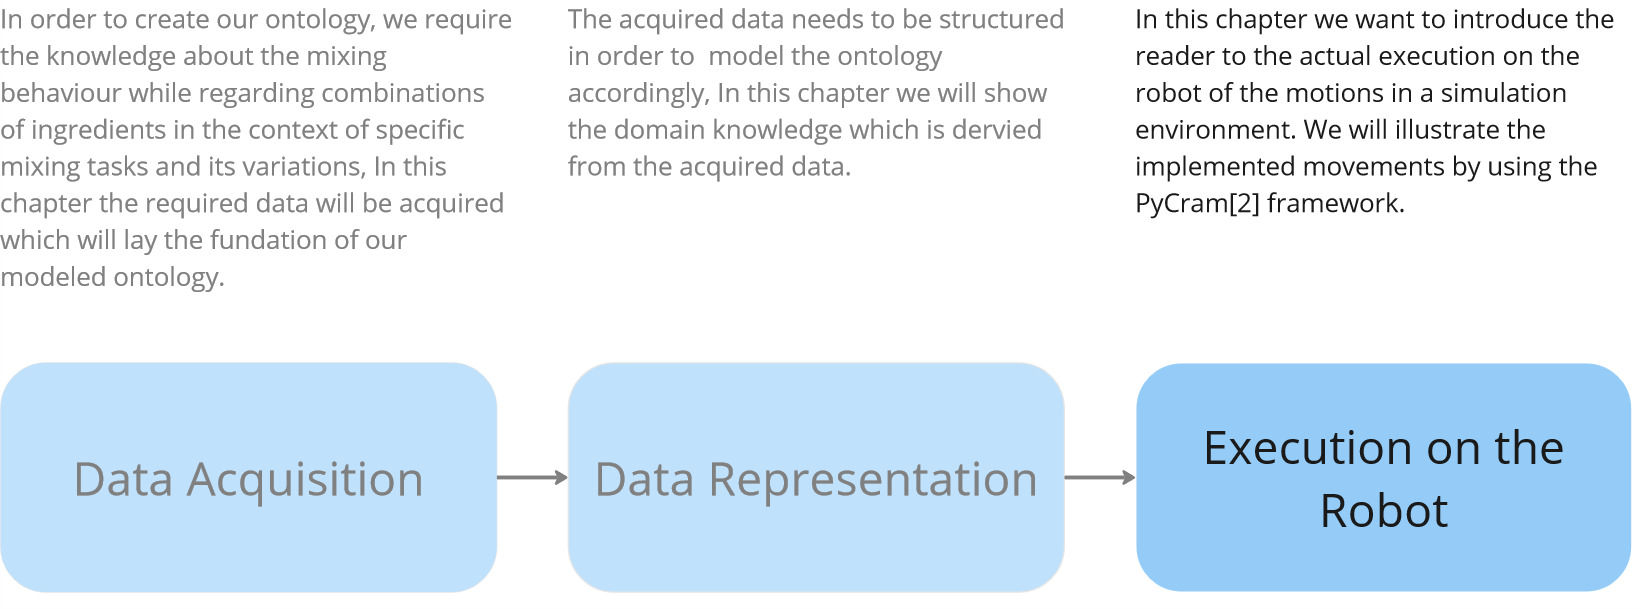
\includegraphics[scale=0.25]{Graphics/structure_overview3.jpg}
\end{figure}
In our work, we have created a knowledge base that can infer parameters to enable an agent to perform various actions.
Since testing these actions on a real robot proves to be challenging, we do so in a simulation.
This chapter aims to provide an overview of the \nameref{sec:simulation environment} in which we test our work and present it as a proof of concept.
Initially, we will explain the environment, including objects, followed by an overview of the motion primitives.
Finally, we will showcase some of our motions (in \nameref{sec:simulated motions}) and discuss the \nameref{sec: simulation to real world gap} before evaluating every motion as a proof of concept and drawing a conclusion where we discuss existing challenges.

\section{Simulation Environment}
\label{sec:simulation environment}

We utilize the simulation environment \textit{BulletWorld} (\ref{sec:pybullet}), which is already integrated into the framework \hyperref[sec:pycram]{PyCRAM} \cite{pycram} . 
In this environment, physics is simulated, which is advantageous for executing the motions we have defined or customized. Additionally, leveraging the \textit{PyCRAM} \cite{pycram} framework allows us to utilize various existing control primitives, such as \textit{Pick and Place}. Communication between the simulation and framework is facilitated by \hyperref[sec:ROS]{ROS} \cite{ros} , which communicates via various nodes, each representing a joint, for instance. Through these nodes, one can obtain information about the joints or transmit commands to modify the parameters of the joints accordingly.


The agent that will execute the various motions in the simulation is the \hyperref[sec:pr2]{PR2} \cite{pr2}.
This robot model has 2 movable arms, as one hand executes the motion. In addition to the fact that the \textit{PR2} \cite{pr2} model is already available in the \textit{PyCram} \cite{pycram} framework,
the \textit{PR2} \cite{pr2} model also has enough joints and degrees of freedom to execute the motions we have adapted.

The agent operates in a kitchen-like environment, the model of which is already included in the \textit{PyCRAM}-core \cite{pycram} and therefore particularly suitable for our use case. The kitchen also features elements such as drawers that can be opened, which are part of real world interactions. Additionally, the kitchen model includes a table on which the agent's actions are ultimately executed. Other furniture is also present in this environment, but is not relevant to our use case.

\begin{figure}[H]
    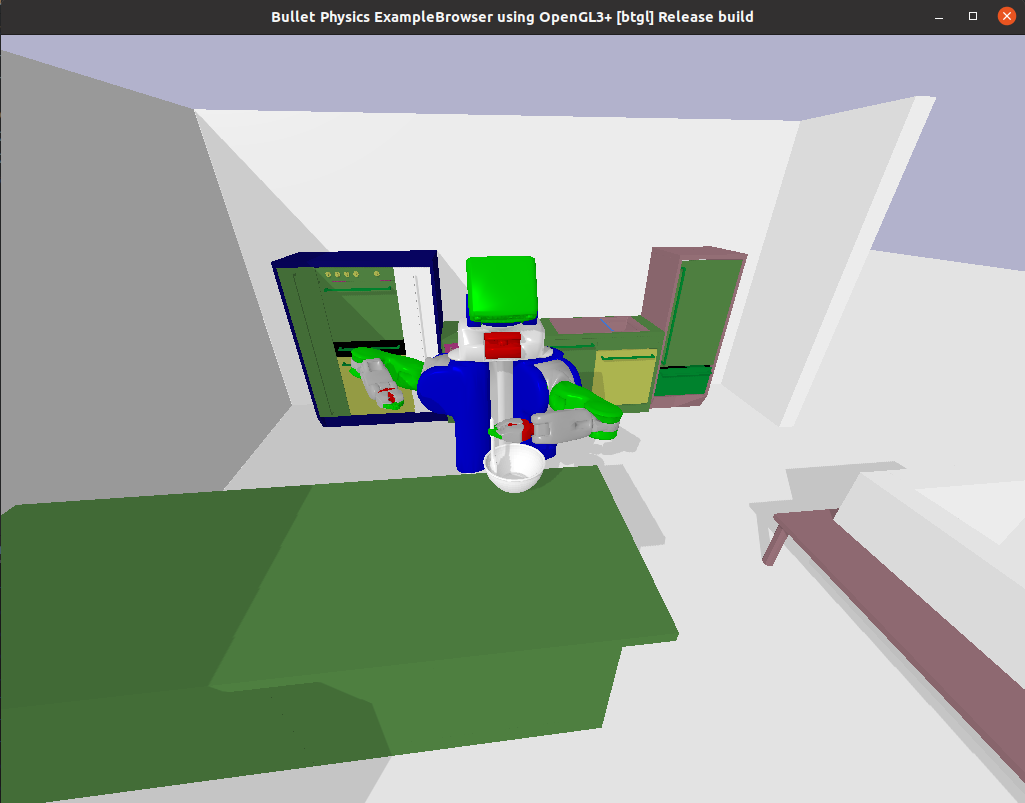
\includegraphics[scale=0.35]{Graphics/bulletworldexample.png}
    \label{fig:bulletworldexample}
    \caption{Simulation Environment containing the \textit{PR2} and \textit{Kitchen} models. }
\end{figure}

For the simulation, we use the objects that have also been defined in the ontology (see \hyperref[sec:ContainersAndToolsAcquisition]{Containers and Tools Acquisition}).
The following objects are available:
\begin{itemize}
	\item Container: 
        \begin{itemize} 
            \item \textit{Small and Large Bowls} - Defined in the ontology as \textit{SaladBowl} and \textit{PastaBowl}
            \item \textit{Pan}
            \item \textit{Pot}
            \item \textit{Cup}
            \item \textit{Mug}
        \end{itemize}
	\item Tools: 
        \begin{itemize}
            \item \textit{Whisk}
            \item \textit{Spoon}/\textit{Wooden Spoon}
            \item \textit{Fork}
        \end{itemize}
\end{itemize}

\begin{figure}[H]
    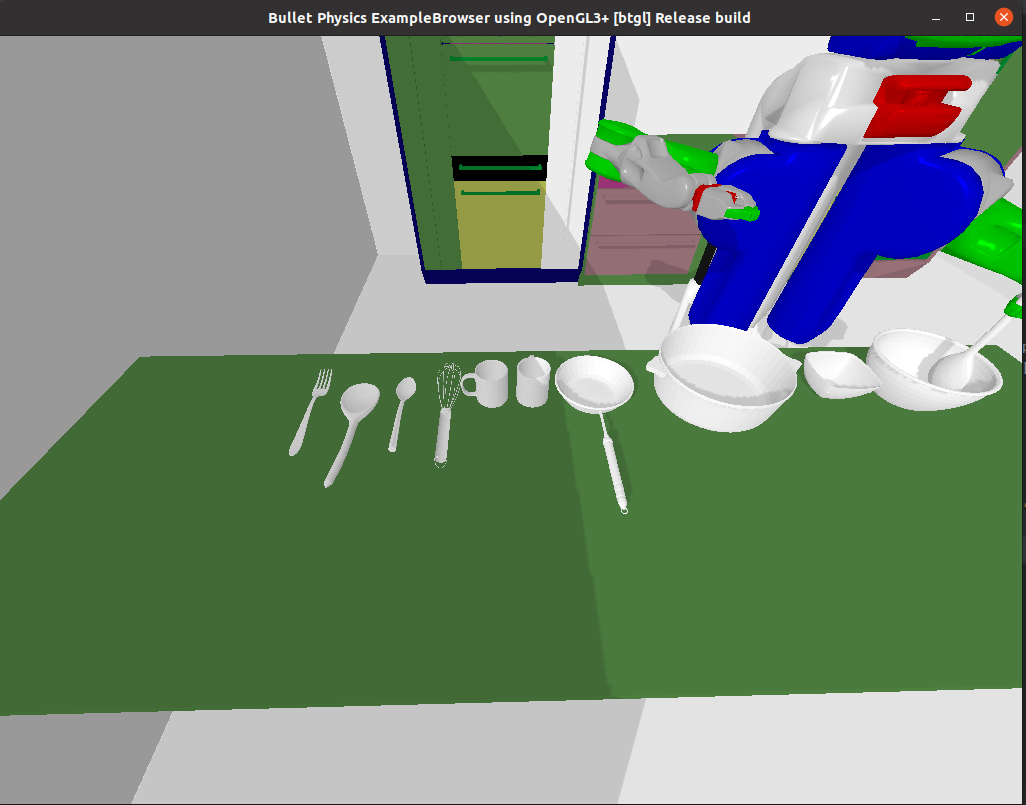
\includegraphics[scale=0.35]{Graphics/toolscontainersmodels.png}
    \label{fig:toolscontainersmodels}
    \caption{Used models for the simulation: \textit{Fork, WoodenSpoon, Spoon, Whisk, Mug, Cup, Pan, Pot, Small Bowl, Big Bowl}}
\end{figure}
In the simulation environment there are no models of ingredients included. Executing motions in the simulation is done as if the motion is executed in 
the vacuum, physical laws regarding ingredient interaction do not apply. The set of ingredients are nonetheless relevant because those ingredients have to be mixed.
\section{Control Primitives}
The framework \nameref{sec:pycram} \cite{pycram} offers a variety of pre-implemented control primitives. These primitives can be used as building blocks to structure the entire execution of a task. These primitives are also defined as \textit{Action Designators}, and the following ones are relevant for our use case:

\begin{lstlisting}
	NavigateAction(target_locations=[pickup_pose.pose]).
					resolve().perform()
\end{lstlisting}
\begin{lstlisting}
	PickUpAction(object_designator_description=tool_object,
                 arms=pickup_pose.reachable_arms,
                 grasps=["top"]).resolve().perform()
\end{lstlisting}

\begin{lstlisting}
	NavigateAction(target_locations=[nav_pose]).
					resolve().perform()
\end{lstlisting}

\begin{lstlisting}
	LookAtAction(targets=[container_object.resolve().pose]).
					resolve().perform()
\end{lstlisting}

\begin{lstlisting}
	MixingActionSWRL(
		object_designator_description=container_object,
        object_tool_designator_description=tool_object,
		ingredients=[Set of Ingredients],
        task="given task",
        arms=["left"],
        grasps=["top"]).parameters_from_owl().perform()
\end{lstlisting}

The last \textit{Action Designator} is a modified version of the existing \textit{Mixing Action Designator}, which has been adapted for our purposes. This designator receives as parameters a container object and a tool object (both not significant for inference), as well as a set of ingredients and a task, which are significant for inference. The performed motion results from the inference together with the applied parameters.

\begin{figure}[H]
    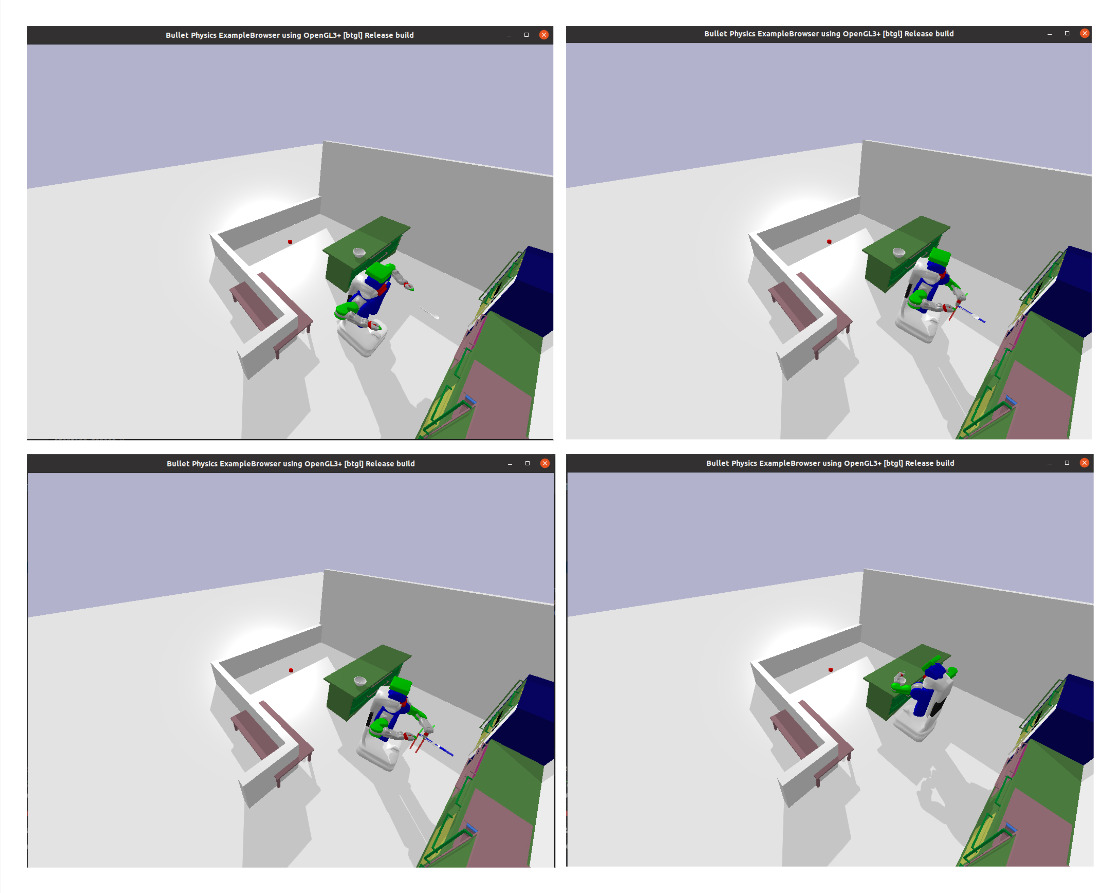
\includegraphics[scale=0.3]{Graphics/control_primitives.jpg}
    \label{fig:controlprimitives}
    \caption{Feautured \textit{Control Primitives}}
\end{figure}

\section{Implementation in PyCram}

\subsection{Robots Plan Execution}
The robots plan used for implementing the MixingActionDesignator and its evaluation is 
a simple plan, including the following steps:

\begin{itemize}
    \item Park Arms
    \item Elevate the robots torso
    \item Navigate to the tool used for mixing
    \item Pick up tool
    \item Park arms
    \item Move to kitchen counter
    \item Look at the container to mix the ingredients
    \item Mix ingredients
\end{itemize}

In the following subsections we will explain, how the robot uses its knowledge during task execution, 
to mix. 

\subsection{Asserted Knowledge}
Any robot capable of executing mixing motions need to have knowledge before executing a mixing task. 
The robot needs to know where the container and tools are located, for picking up and for navigation to Theoretically
respective places. It needs to know which ingredients have to be mixed, in simulation only their existence have to be known. 
It needs to know which task to execute, since we differentiate between different mixing tasks as discussed in this section. 


\subsection{Inferring Knowledge}
As of now, the robot doesn't know what kind of mixing motion it has to perform. Its associated parameters are also unknown. 
Therefore, the robot needs to reason about its assertional knowledge.
Once it has access to all relevant information, it can infer the appropriate mixing motion or motions, in case a compound motion has been
inferred, with its corresponding parameters through logical reasoning.
Logical reasoning is performed inside the custom resolver \textit{MixingActionSWRL}.

\subsection{MixingActionSWRL}
\label{subsection:MixingActionSWRL}
\textit{MixingActionSWRL} is a custom resolver using our \textit{mixing} ontology to infer motions from the robots assertional knowledge.
The resolvers task is to fill the missing descriptions of which motions should be executed with its associated parameters.

\paragraph{Initialization}
The resolver loads the mixing ontology, creates \textbf{NamedIndividuals} of the task to execute and of all ingredients which are being mixed.
Since we wanna infer facts from SWRL rules, every actor in the mixing process has to be created as a \textbf{NamedIndivuidual} 
All names need to be available for later instantiation.
A \textbf{NamedIndividual} is created from the high level class \textit{Motion}, representing the individual of all possible motions. 
The resolver attempts to reclassify this motion into a specific motion that is going to be executed on the robot.

First container, tool and ingredients are instantiated, additionally a task instance is created and its relations with 
the other individuals are assigned. To find the proper corresponding class, to the names of the container, ingredients, task and tool
we perform fuzzy string matching to find a matching class to the name. 

\paragraph{Fuzzy String Matching}
Using the levenshtein distance, syntactic similarity of two different strings is computed. A low distance score
indicates a higher similarity than a high score. However, this metric does not account for semantic similarities, 
as the words meanings are not considered in the computation of distance.

\paragraph{Inference}
Once the relations have been assigned, using \textit{OWLReady} with builtin functions calling reasoners like \textit{Pellet} or \textit{HermIt},
reclassifies the motion instance using the defined \textit{SWRL} rules inside the \textit{mixing} ontology.
Since the individual instantiated from the class \textit{Motion} has been reclassified the motion parameters can be extracted from the class.

Finally, the resolver completes the sequence of motions to be executed with its associated parameters and 
forwards it to the MixingAction.

\subsection{MixingActionDesignator}
The \textit{MixingActionDesignator} is a newly implemented action designator 
designed to perform various types of mixing motions or sequences of motions within a specific container using a specific tool. 
This designator generates poses that follow a trajectory, simulating the process of mixing in the bulletworld environment.
To effectively break down the action into executable motions, certain designator descriptions are required.

\subsection{Implementation}

\paragraph{Designator Description}
\begin{enumerate}
    \item \textit{Container Object Designator}:
    \begin{itemize}
        \item This object designator contains information about its name and its bulletword internal represnation.
            Its bulletworld representations holds information like the current objects pose and its 3D axis aligned bounding box.
            This bounding box can be used to compute the dimensions of the container along each axis. 
            Knowing the bounds and the pose of the container is crucial, because the motion has to performed inside 
            the container within its boundaries.
    \end{itemize}
    \item \textit{Tool Object Designator}:
    \begin{itemize}
        \item Analogous to the container this designator contains the same type of information.
        Knowing the dimensions of the tool is crucial in avoiding collision with the container.
    \end{itemize}
    \item \textit{Arm}:
    \begin{itemize}
        \item Which arm should be used to perform the mixing action
    \end{itemize}
    \item \textit{Motions}:
    \begin{itemize}
        \item A list of motions as strings to be performed. 
    \end{itemize}
    \item \textit{Motion Parameters}:
    \begin{itemize}
        \item Each motion has its own key value pairs of parameters.
        These parameters alongside the motion are resolved by the \nameref*{subsection:MixingActionSWRL}
    \end{itemize}
\end{enumerate}

\paragraph*{Resolving motion and parameters}
The \textit{MixingActionDesignator} calls the \textit{MixingActionSWRL} resolver, to infer the motion with its 
associated parameters. 

\paragraph*{Sequential Processing in MixingActionDesignator}
Once all descriptions are available for the \textit{MixingActionDesignator}, it attempts the following steps in sequence:

\begin{enumerate}
    \item \textbf{Retrieve BulletWorld Objects}: The BulletWorld objects for both the container and the tool are retrieved from the object designator. 
    Each BulletWorld object has a 3D axis-aligned bounding box. Using this bounding box, the dimensions can be computed. 
    The implemented function \textit{get\_object\_dimensions()} returns the three dimensions of each BulletWorld object.
    \item \textbf{Motions}: Access the motion names and find out which motion has to be executed.
    \item \textbf{Calculate Radius Bounds}: The upper and lower radius bounds, which are relative values, 
    are accessed to compute the absolute radius for the respective mixing motion, using the dimensions of container and tool, to ensure
    that any mixing motion is executed inside the container.
    \item \textbf{Transform Container Pose}: The container's pose is retrieved and transformed into its own coordinate frame from the world coordinate frame to 
    compute mixing poses fitted to the container in its coordinate frame.
    \item \textbf{Generate Motion Trajectory}: Based on the current motion, 3D coordinates are generated using the functions defined in the section \nameref{sec:Motions},
    the values inside the motion parameters list are used for computation.
    \item \textbf{MoveTCP}: For each generated pose, that pose is elevated by a constant value and the execution of motion is done with MoveTCP, which 
    moves the tool center point of the robots arm.
    
\end{enumerate}
\subsection{Simulated Motions}
\label{sec:simulated motions}

This section will illustrate the results of our implemented motions in the \textit{MixingActionDesignator}. 
We will contrast each motion with a plot and a picture, which contain the generated poses with their visualized axes.

\subsubsection{Whirlstorm Motion}

\begin{figure}[H]
    \centering
    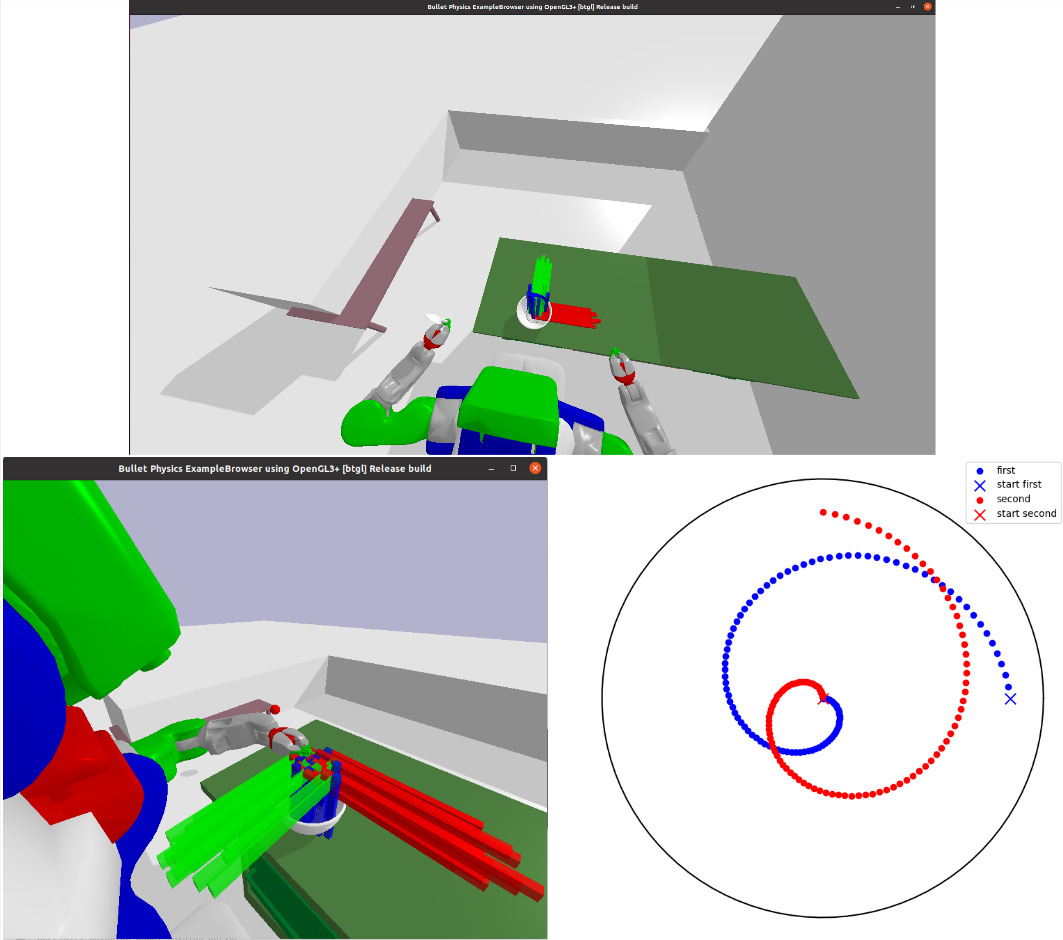
\includegraphics[scale=0.27]{Graphics/whirlstorm_showcase.jpg}
    \caption{Feautured \textit{Whirlstorm Motion}}
    \label{fig:whirlstormshowcase}
\end{figure}



\subsubsection{Circular Motion}

\begin{figure}[H]
    \centering
    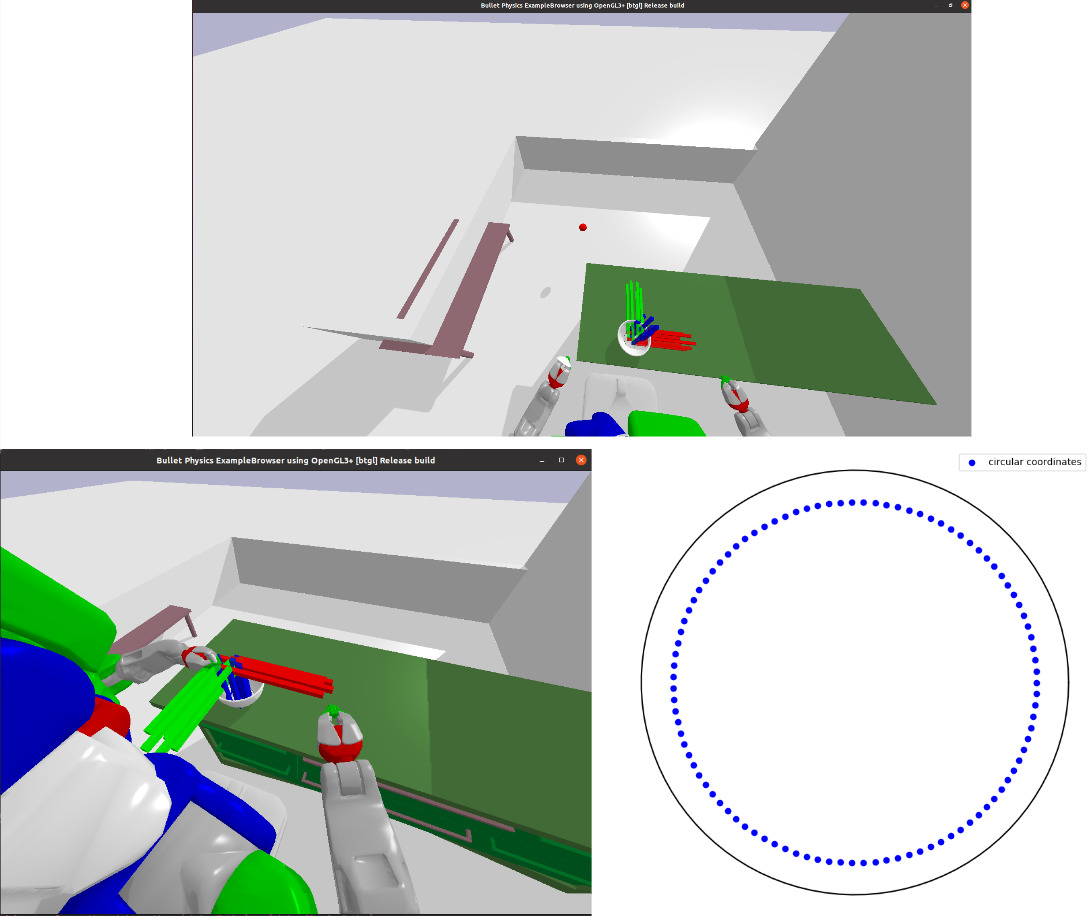
\includegraphics[scale=0.27]{Graphics/circular_showcase.jpg}
    \caption{Feautured \textit{Circular} Motion}
    \label{fig:circularshowcase}
\end{figure}


subsubsection{Horizontal Eliptical}
\begin{figure}[H]
    \centering
    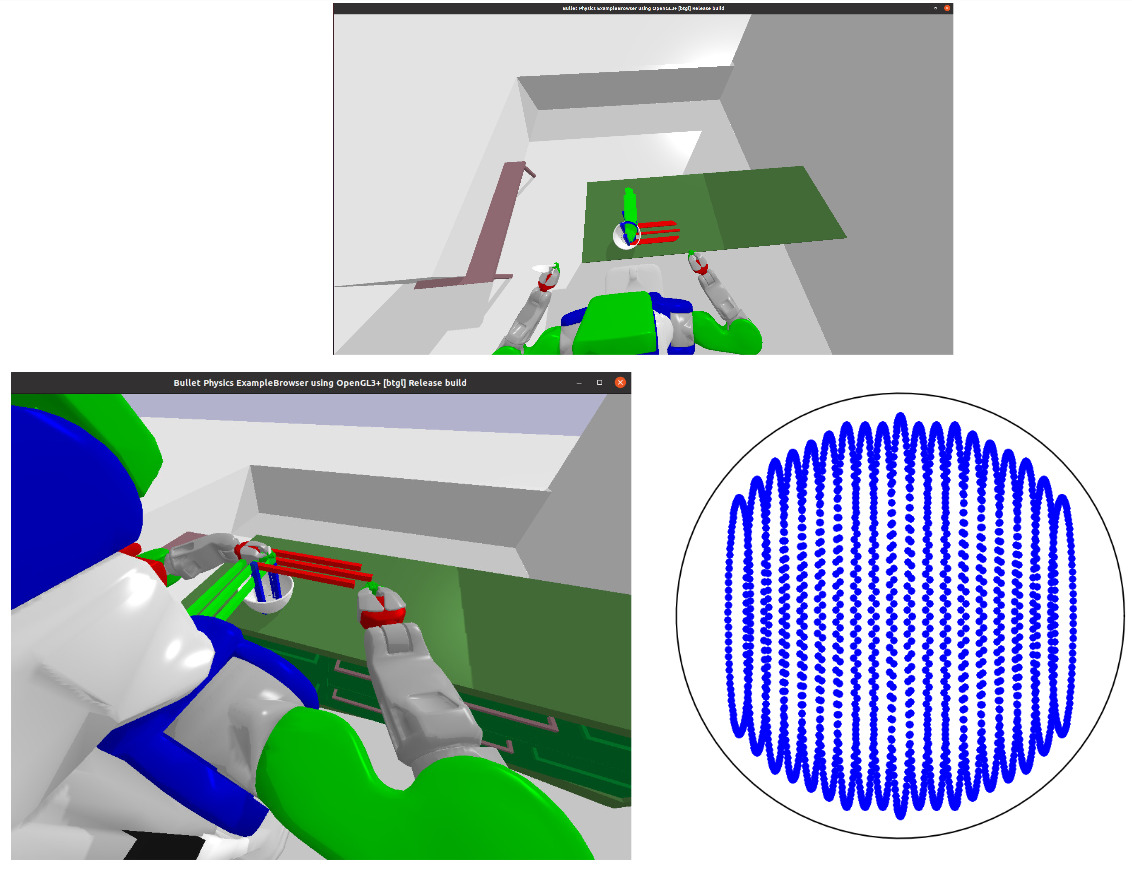
\includegraphics[scale=0.27]{Graphics/horizontal_showcase.jpg}
    \caption{Feautured \textit{Horizontal Eliptical} Motion}
    \label{fig:circularshowcase}
\end{figure}

subsubsection{Folding Motion}
\begin{figure}[H]
    \centering
    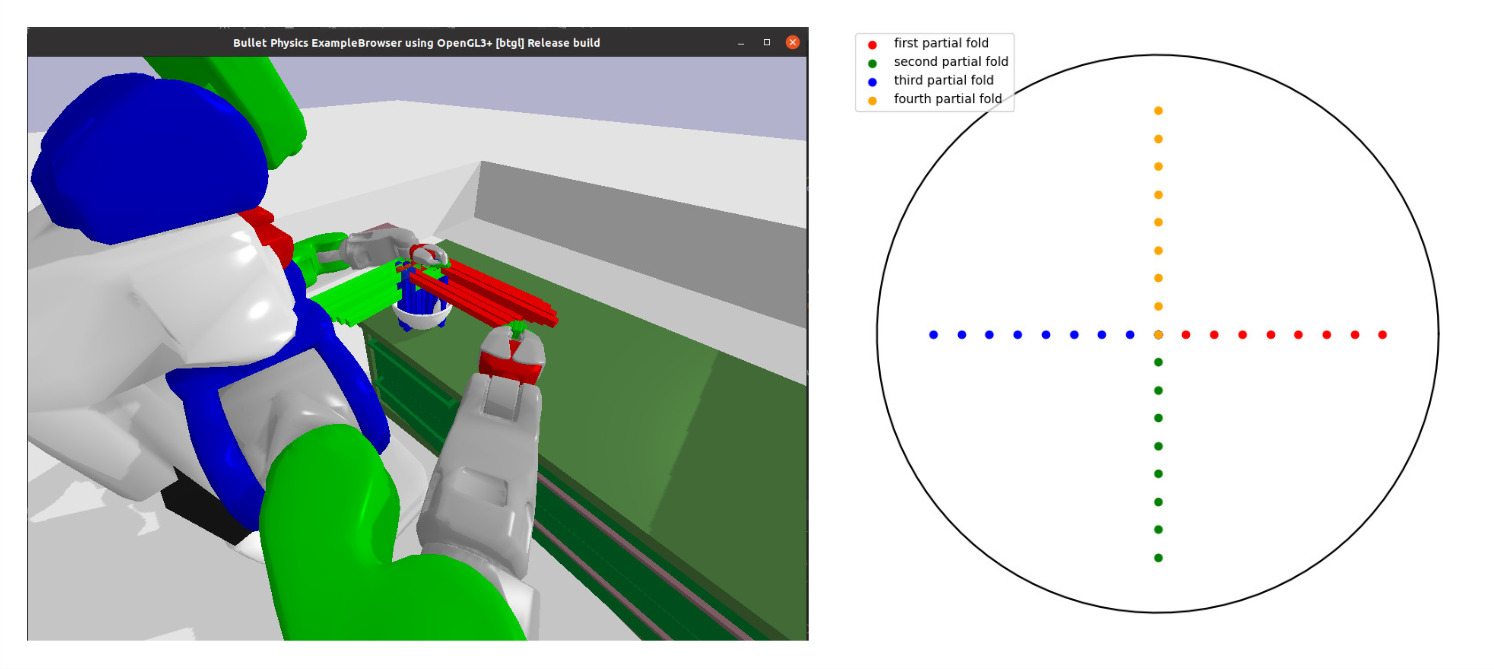
\includegraphics[scale=0.27]{Graphics/folding_showcase.jpg}
    \caption{Feautured \textit{Folding} Motion}
    \label{fig:foldingshowcase}
\end{figure} 

\section{Simulation to Real-World Gap}
\label{sec: simulation to real world gap}
Robots operating in the kitchen domain face numerous challenges when using the \textit{MixingActionDesignator} in real-world scenarios. 
Unlike in simulations, where each executed movement of the mixing action follows precise trajectories, 
the complexity of executing mixing tasks and their associated motions in real-world conditions rises tremendously. 
The \textit{MixingActionDesignator} lacks any form of failure handling to address potential challenges in real-world scenarios

When mixing different ingredients in the real world, the physical properties of the ingredients must be considered, 
as the motion can no longer be executed in a vacuum. Properties such as viscosity, density, 
and texture will influence the ability to mix these ingredients, potentially leading to inefficient mixing and 
unsatisfactory results for the user. 
The mixing process is further complicated by the mechanical limitations of the robot, 
where applied force, speed, and other characteristics will affect the outcome.

A robotic system relying on ground truth loses this certainty when transitioning to the real world, 
encountering various types of uncertainty instead. 
The robot loses knowledge about the locations of ingredients, tools, and containers. 
Consequently, it requires a functioning perception system capable of identifying and locating objects in a scene. 
Additionally, the computation of object boundaries must be done via approximation, which is a critical requirement for the \textit{MixingActionDesignator}.

The robot's ability to perceive all required objects for the mixing task can be limited by 
visual phenomena such as poor lighting conditions, reflections, occlusions, and other visual challenges. 
Moreover, the inherent variability in the appearance and shape of ingredients can challenge object recognition algorithms, resulting in misidentification or ambiguity.

In real world scenarios, object poses are no longer known to the robot, 
making reliable pose estimation essential. 
A good grasp pose is crucial for all objects to ensure they are picked up properly and transported safely to their destination. 
For instance, a tool should generally be picked up by the handle rather than the head to ensure proper handling. 
Without accurate pose estimation, the robot might misalign with objects, leading to failed grasp attempts, dropped items,
or even damage to the objects or the robot itself. The variability in object shapes, sizes, 
and textures requires the robot to continuously adapt its grasping strategy, further emphasizing the need for precise and reliable pose estimation 
to maintain efficiency and accuracy in the task.

\section{Challenges and Difficutlies, Summary of the Simulation}
Overall, we are satisfied with the results of the simulation. In the following section \nameref{sec:evaluation}, the various motions are tested and evaluated with different combinations of tasks, ingredients, tools, and containers. One point we would like to address is the initially planned motions, which have a height increment, meaning the motions would not only be executed in 2 dimensions but in 3. Implementing this in the simulation proved to be challenging, so we decided against further consideration of these motions due to the effort involved.

At the current state the robot in simulation either succesfully executes actions or fails to do so.
In case of failues there is no recovery to succesfully execute a mixing task. The robot is not able critically
reflect upon its made failures.
